\section{Загальні принципи використання стилів оформлення у текстовому процесорі \LaTeX{}}
\subsection{Стилі у \LaTeX{}}
\subsubsection{Загальні положення}

Стилі допомагають встановлювати оформлення для обраних елементів тексту. Оформлення включає:
\begin{itemize}
\item гарнітуру, розмір та особливості напису шрифту;
\item параметри абзацу, такі як відступи, міжстрочний інтервал, положення на сторінці;
\item нумерація або маркування списків;
\item колір шрифту або фону;
\item та інше.
\end{itemize}

В \LaTeX{} неможливо обійтися без стилів, команд та оточень. Навіть виправлення
помилки оформлення в одному місці вимагає правки стиля усього документа.

\subsubsection{Команди та оточення, що реалізовані у шаблоні}

Для реалізації вимог стандарта або застосовується спеціальна команда чи оточення
(див.~\label{sec:auto}) або виконуються допоміжні дії по редагуванню документа
(див.~\label{sec:manual}). 

Перелік оточень включає:
\begin{enumerate}
\item stdfigure;
\item itemize;
\item enumerate;
\item longEnumerate;
\item description;
\item formulaDescription;
\item abbrDescription;
\item equation;
\item equation*;
\item stdtableshort;
\item stdtablelong.
\end{enumerate}

Перелік команд включає:
\begin{enumerate}
  \item section, subsection, subsubsection;
  \item footnote;
  \item item (тільки всередені оточень itemize, enumerate, longEnumerate,
  description, formulaDescription, abbrDescription);
  \item cite;
  \item label + ref.
\end{enumerate}

\subsubsection{Пункти стандарту, що враховуються автоматично}\label{sec:auto}

Перелік пунктів стандарту, що можуть бути автоматично виконані призначенням відповідного стилю:
\begin{enumerate}
\item текст документа (п.4.3);
\item зміст (п.5.3) генерується автоматично (на базі команд section, subsection, subsubsection)
\item перелік джерел інформації (п.5.8) реалізується за допомогою bibTeX;
\item переліки (п.6.2.7-6.2.10) реалізуються ко, при цьому:
\begin{itemize}
  \item оточення longEnumerate використовується коли у пунктах (хоча би одному) більш ніж одне речення; при цьому перед переліком ставиться крапка, в кінці кожного пункту ставиться крапка;
  \item оточення enumerate використовується коли у кожному пункті одне речення, при цьому в кінці кожного пункту ставиться крапка з комою а кінці останнього пункту ставиться крапка;
\end{itemize}
\item заголовки структурних підрозділів (п.6.2.11-6.2.15) реалізуються командами section, subsection, subsubsection;
\item розташування формул (пп.6.3.2.1-6.3.2.3) реалізуються оточеннями equation* (формула без номера) та equation (формула з номером);
\item пояснення позначень у формулах (п. 6.3.2.4) реалізуються оточенням formulaDescription;
\item вставка рисунку (п. 6.3.4) реалізується оточенням stdfigure, підпис, та розташування проводиться автоматично.
\end{enumerate}

Деякі пункти стандарту виконуються автором самостійно. Приклади оформлення представлені у наступних розділах.

\subsection{Пункти стандарту, які треба враховувати самостійно}

6.2.6 Якщо розділ або підрозділ поділено на пункти (або пункт поділено на підпункти), то включення у цей розділ, підрозділ (пункт) тексту, що передує першому пункту (підпункту) не допускається.

6.2.10 \dots (довгі нумеровані списки) починають з великої літери і відокремлюють один від одного крапкою \dots

6.2.11 \dots Заголовки (найменування) розділів, підрозділів, пунктів, підпунктів мають відображати їх зміст та бути короткими і точними. Крапку у кінці заголовка не ставлять. Якщо заголовок складається з двох речень, їх розділяють крапкою. \dots

\subsection{Відомі проблеми}

\begin{longEnumerate}
\item Стилі таблиць коректно працюють лише для широких таблиць (на всю область сторінки). Інакше, заголовок таблиці всеодно відображається ліворуч, а не над першою колонкою таблиці.
\item В Footnote не працює одинарний інтервал (залишається півтора) 
\end{longEnumerate}

\section{Нотатки по практичному застосуванню шаблона}
\subsection{Оформлення списку джерел інформації}

Оформлення списку джерел інформації проводиться згідно ДСТУ ГОСТ 7.1:2006
«Бібліографічний запис, бібліографічний опис. Загальні вимоги та правила
складання»~\cite{DSTU_GOST_7.1_2006}. Приклади оформлення джерел наведені у
даному документі.

\subsection{Використання команд і оточень}
\subsubsection{Списки}

Маркірований список

\begin{framed}\small
\begin{lstlisting}
\begin{itemize}
\item one;
\item two;
\item three.
\end{itemize}
\end{lstlisting}
\end{framed}

\begin{itemize}
\item one;
\item two;
\item three.
\end{itemize}

Нумерований список

\begin{framed}\small
\begin{lstlisting}
\begin{enumerate}
\item one;
\item two;
\item three.
\end{enumerate}
\end{lstlisting}
\end{framed}

\begin{enumerate}
\item one;
\item two;
\item three.
\end{enumerate}

Нумерований розгорнутий список

\begin{framed}\small
\begin{lstlisting}
\begin{longEnumerate}
\item Lorem ipsum dolor sit amet, consectetur adipiscing elit. 
 Nam euismod semper arcu, id tempor ligula pellentesque sed.
\item Integer quis metus sapien, at auctor ipsum. Pellentesque
 scelerisque lacinia nisi vestibulum eleifend.
\item Aenean vel nunc tortor, ac facilisis mauris. Phasellus
 sed quam risus, vel dictum nibh.
\end{longEnumerate}
\end{lstlisting}
\end{framed}

\begin{longEnumerate}
\item Lorem ipsum dolor sit amet, consectetur adipiscing elit. Nam euismod semper arcu, id tempor ligula pellentesque sed. 
\item Integer quis metus sapien, at auctor ipsum. Pellentesque scelerisque lacinia nisi vestibulum eleifend. 
\item Aenean vel nunc tortor, ac facilisis mauris. Phasellus sed quam risus, vel dictum nibh.
\end{longEnumerate}

Вкладені списки

Маркірований список вкладений до нумерованого

\begin{framed}\small
\begin{lstlisting}
\begin{enumerate}
\item one;
\item two:
\begin{itemize}
  \item two one;
  \item two two;
  \item two three.
\end{itemize}
\item three.
\end{enumerate}
\end{lstlisting}
\end{framed}

\begin{enumerate}
\item one;
\item two:
\begin{itemize}
  \item two one;
  \item two two;
  \item two three.
\end{itemize}
\item three.
\end{enumerate}

Маркірований список вкладений до нумерованого розгорнутого

\begin{framed}\small
\begin{lstlisting}
\begin{longEnumerate}
\item Lorem ipsum dolor sit amet, consectetur adipiscing elit.
 Nam euismod semper arcu, id tempor ligula pellentesque sed.
\item Integer quis metus sapien, at auctor ipsum. Pellentesque
 scelerisque lacinia nisi vestibulum eleifend:
\begin{itemize}
  \item two one;
  \item two two;
  \item two three.
\end{itemize}
\item Aenean vel nunc tortor, ac facilisis mauris. Phasellus
 sed quam risus, vel dictum nibh.
\end{longEnumerate}
\end{lstlisting}
\end{framed}

\begin{longEnumerate}
\item Lorem ipsum dolor sit amet, consectetur adipiscing elit. Nam euismod semper arcu, id tempor ligula pellentesque sed. 
\item Integer quis metus sapien, at auctor ipsum. Pellentesque scelerisque
lacinia nisi vestibulum eleifend:
\begin{itemize}
  \item two one;
  \item two two;
  \item two three.
\end{itemize}
\item Aenean vel nunc tortor, ac facilisis mauris. Phasellus sed quam risus, vel dictum nibh.
\end{longEnumerate}

Нумерований літерами

\begin{framed}\small
\begin{lstlisting}
\begin{enumerate}
\item one;
\item two:
\begin{enumerate}
  \item two one;
  \item two two;
  \item two three;
  \item two four;
  \item two five;
  \item two six;
  \item two seven;
  \item two eight;
  \item two nine;
  \item two ten.
\end{enumerate}
\item three.
\end{enumerate}
\end{lstlisting}
\end{framed}

\begin{enumerate}
\item one;
\item two:
\begin{enumerate}
  \item two one;
  \item two two;
  \item two three;
  \item two four;
  \item two five;
  \item two six;
  \item two seven;
  \item two eight;
  \item two nine;
  \item two ten.
\end{enumerate}
\item three.
\end{enumerate}

Інші варіанти не підтримуються.

\subsubsection{Вставка формул}

Для вставки формули з номером:

\begin{framed}\small
\begin{lstlisting}
\begin{equation}
\text{ Це } \Delta =\sum_{i=1}^N w_i (x_i - \bar{x})^2 .
\end{equation}
\end{lstlisting}
\end{framed}

Результат:

\begin{equation}
\text{ Це } \Delta =\sum_{i=1}^N w_i (x_i - \bar{x})^2 .
\end{equation}

Для вставки формули без номеру

\begin{framed}\small
\begin{lstlisting}
\begin{equation*}
g = \frac{1}{2} \sqrt{2\pi}
\end{equation*}
\end{lstlisting}
\end{framed}

Результат:

\begin{equation*}
g = \frac{1}{2} \sqrt{2\pi}
\end{equation*}

Змінні що використані у формулі та не були описані до того у тексті повинні бути
описані відразу після формули. 

\begin{framed}\small
\begin{lstlisting}
\begin{equation}
E = -J \sum_{i=1}^N s_i s_{i+1} ,
\end{equation}
# leave an empty line here

\begin{formulaDescription}
\item[$E$] something;
\item[$J$] something else.
\end{formulaDescription}
\end{lstlisting}
\end{framed}

Результат:

\begin{equation}
E = -J \sum_{i=1}^N s_i s_{i+1} ,
\end{equation}

\begin{formulaDescription}
\item[$E$] something;
\item[$J$] something else.
\end{formulaDescription}

\subsubsection{Оформлення ілюстрацій}

\begin{framed}\small
\begin{lstlisting}
\begin{stdfigure}
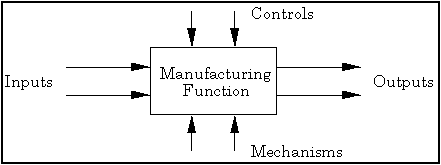
\includegraphics[width=2.7in]{images/idef_fb.png}
\caption{Figure caption}
\label{fig:idef_fb}
\end{stdfigure}
\end{lstlisting}
\end{framed}

Результат:

\begin{stdfigure}
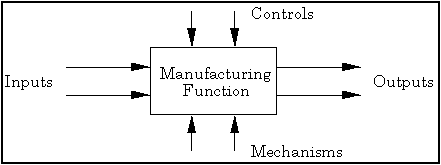
\includegraphics[width=2.7in]{images/idef_fb.png}
\caption{Figure caption}
\label{fig:idef_fb}
\end{stdfigure}

Оформлення рисунків, що переносяться між сторінками досі не підтримується даним
шаблоном (хоча частково відповідний код вже написано).

\subsubsection{Оформлення таблиць}

Короткі таблиці

\begin{framed}\small
\begin{lstlisting}
\begin{stdtableshort}{2}{|c|c|}
{\label{tbl:shorttbl}Short table name}
{
Lorem &
Ipsum
}
1 & 2 \\ \hline
3 & 4 \\ \hline
\end{stdtableshort}
\end{lstlisting}
\end{framed}

Довгі таблиці, що переносяться на декілька сторінок

\begin{framed}\small
\begin{lstlisting}
\begin{stdtablelong}{2}{|c|c|}
{\label{tbl:ndrparam}Long table name}
{
Lorem &
Ipsum
}
1 & 2 \\ \hline
% insert table rows here 
99 & 100 \\ \hline
\end{stdtableshort}
\end{lstlisting}
\end{framed}

\subsubsection{Оформлення додатків}

\begin{framed}
\begin{lstlisting}
\startAppendix
\appendixSection{Addon 1}\label{add:addon1} 
\appendixSubsection{Subsection header}
\appendixSubsubsection{Subsubsection header}
\end{lstlisting}
\end{framed}

Приклад наведено у додатку \ref{add:addon1}.

\subsection{Робота зі стилями}

Основні стилі зберігаються у файлі stvuz\_khpi.cls.
Його вихідний код наведено у додатку \ref{add:source}. При необхідності, можна
додавати стилі в преамбулу документу.

\subsection{Титульниі листи}

Рекомендується виконувати титульні листи в окремому документі, наприклад, в
текстових процесорах Libre Office чи Microsoft Office Word, тому що їх
оформлення вимагає більшої кількості нестандартних стилів.

\subsection{Можливі проблеми та підходи до їх розв'язання}

Проблеми використання розробленого шаблону мають різне походження.

Якщо щось не так - спробуйте погратися доданням чи видаленням тексту, переносів
сторк.

\begin{longEnumerate}
\item \ldots 
\end{longEnumerate}

\section{Приклади використання стилів}

\subsection{Огляд методів моделювання й опису процесів}
\subsubsection{Загальні положення}
Моделі виробничих процесів можна класифікувати в наступному виді:
\begin{itemize}
\item описові;
\item алгоритмічні;
\item математичні;
\item \dots~.
\end{itemize}

Математичні моделі ...

\subsubsection{Методи імітаційного моделювання}
Імітаційна модель~-- це математична модель, що відбиває істотні для дослідника особливості досліджуваної системи.

Імітаційні моделі створюються для рішення наступних завдань:
\begin{enumerate}
\item визначення реакції складної системи на керуючий вплив у ситуації, коли безпосередні експерименти з нею дорогі, складні, або небезпечні;
\item \dots
\item в інших ситуаціях, що вимагають попередньої оцінки наслідків прийнятих
рішень\footnote{Розглядається множина що \ldots Розглядається множина що
Розглядається множина що Розглядається множина що Розглядається множина що
Розглядається множина що}:
\begin{itemize}
\item перша ситуація;
\item інша ситуація.
\end{itemize}
\end{enumerate}
У цей час використаються наступні інструментальні засоби імітаційного моделювання.
\begin{longEnumerate}
\item Система імітаційного моделювання GPSS. Це потужне середовище комп'ютерного моделювання загального призначення, розроблене для професіоналів в області моделювання. 
\item Це комплексний моделюючий інструмент, що охоплює області як дискретного, так і безперервного комп'ютерного моделювання, що має високий рівень інтерактивності й візуального подання інформації.
\item Пакет прикладних програм MATLAB. Призначений для рішення завдань технічних обчислень. Включає мову програмування. Використається більш ніж 1000000 інженерних і науковців, і працює на більшості сучасних операційних систем, включаючи:
\begin{itemize}
\item Linux; 
\item Mac OS; 
\item Solaris; 
\item Windows.
\end{itemize}
\item Система ARENA компанії Systems Modeling. Дозволяє будувати імітаційні моделі, програвати їх і аналізувати результати такого програвання, і ін.
\end{longEnumerate}

\subsubsection{Мова специфікації процесів (Process Specification Language)}
[текст пункту]
\subsubsection{Методологія IDEF}
Методологія IDEF (I-CAM DEFinition) розробляється компанією Knowledge Based Systems, Inc\ldots
Стандарт IDEF0 призначений для моделювання
бізнес-функцій~\cite{Sommerville_2010}. Структура функціонального блока в методології IDEF0 приведена на рисунку
\ref{idef_fb}.

\begin{stdfigure}
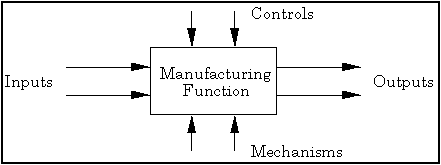
\includegraphics[width=2.7in]{images/idef_fb.png}
\caption{Структура функціонального блоку}
\label{idef_fb}
\end{stdfigure}

\subsection{Функціональний аналіз виробничого процесу зборки регулятора напруги}

Виробничий процес зборки регулятора напруги\ldots

\subsection{Постановка задачі моделювання виробничого процесу зборки регулятора
напруги}

Необхідно розробити імітаційну модель процесу зборки регулятора напруги\ldots

Моделі виробничих процесів можна класифікувати в наступному виді:
\begin{itemize}
\item описові;
\item алгоритмічні;
\item математичні.
\end{itemize}

Математичні моделі [текст пункту]


\subsection{Застосування мереж Петрі до вирішення задачі моделювання
виробничого процесу зборки регулятора напруги} 

\ldots

Мережа Петрі $M = (C, \mu)$ є такою що строго зберігає, коли для всіх маркувань
$\mu' \in R(C, \mu)$ виконується співвідношення

\begin{equation}
\sum_{p_i \in P}{\mu'(p_i)}=\sum_{p_i \in P}{\mu(p_i)}
\end{equation}

\begin{formulaDescription}
\item[$\mu'$] маркування;
\item[$p_i$] перехід мережи.
\end{formulaDescription}

Таким чином, загальна кількість фішок в будь-якому маркуванні із множини
досяжності $R(C, \mu)$ дорівнює загальному числу фішок у початковому маркуванні
$\mu$.

\ldots

Матричне подання мережі Петрі визначає іншу форму основних правил виконання
мережі - правила дозволу переходів і правила зміни маркування. Перехід $t_j \in 
T$ є дозволеним у маркуванні $\mu$, якщо виконується у векторному змісті
співвідношення

\begin{equation}\label{eqn:ejd}
\mu \geq e[j] D
\end{equation}

Оскільки $e[3] D^{-}$ = (0 0 1 0), то співвідношення (\ref{eqn:ejd}) виконується
для переходу t3 $\mu > e[3] D^{-}$. Отже, перехід t3 є дозволеним в
маркуванні $\mu = ( 1 0 1 0 )$.

\ldots

\subsection{Функціональна структура програмного забезпечення із застосуванням
IDEF0-методології}

\ldots

\subsection{Інформаційно-логічна схема програмного забезпечення із застосуванням
IDEF1Х-методологии}

\ldots

\subsection{Посібник користувача програмного забезпечення}

\ldots

\section{Застосування розробленого програмного забезпечення до моделювання
виробничого процесу зборки регулятора напруги}

\subsection{Вхідна й вихідна інформація}

Технологічні характеристики встаткування наведені в додатку А. 

\ldots

На рисунку 4.1 наведено алгоритм обчислення характеристик обладнання.

\subsection{Аналіз отриманих результатів моделювання}

Наводимо результати проведення чисельних експериментів з математичною моделлю (таблиця \ref{tbl:experiment}).


\begin{stdtablelong}{5}{|C{2cm}|C{4cm}|C{4cm}|C{4cm}|C{2cm}|}
{\label{tbl:experiment}Результати
проведення чисельних експериментів з математичною моделлю}
{  
 № варіанта &
\multicolumn{3}{C{12cm}|}{Значення параметрів технологічного встаткування} &
Час зборки, с \\ \cline{2-4}
& A & B & C &
}

1 & & & & \\ \hline
2 & & & & \\ \hline 
3 & & & & \\ \hline
4 & & & & \\ \hline
5 & & & & \\ \hline
6 & & & & \\ \hline
7 & & & & \\ \hline
8 & & & & \\ \hline
9 & & & & \\ \hline
10 & & & & \\ \hline
11 & & & & \\ \hline
12 & & & & \\ \hline
13 & & & & \\ \hline
15 & & & & \\ \hline
16 & & & & \\ \hline
17 & & & & \\ \hline
18 & & & & \\ \hline
19 & & & & \\ \hline
20 & & & & \\ \hline
21 & & & & \\ \hline
22 & & & & \\ \hline
23 & & & & \\ \hline
24 & & & & \\ \hline
25 & & & & \\ \hline
26 & & & & \\ \hline
27 & & & & \\ \hline
\end{stdtablelong}

Результати моделювання наведені в таблиці \ref{tbl:ndrparam} \cite{KuzmenkoSafety}.


\begin{stdtableshort}
  {2}
  {|c|X|}
  {\label{tbl:ndrparam}Характеристика роботи}
  {Час спостережень & Значення параметру}
00:01 & 1 \\ \hline
00:02 & 2 \\ \hline
00:03 & 1 \\ \hline
00:04 & 3 \\ \hline
\end{stdtableshort}


Отже, \ldots
